\documentclass[12pt,letterpaper,spanish]{book}

% formato, lenguaje y encoding
\usepackage[utf8]{inputenc}
\usepackage[T1]{fontenc}
\usepackage[spanish, es-nolists, es-lcroman]{babel}
\usepackage[spanish]{babelbib}
\usepackage[top=3cm, left=3cm, bottom=3cm, right=2cm, paper=letterpaper]{geometry}


% Links y numeracion del PDF
\usepackage[pdfpagelabels]{hyperref}

% Codigo Fuente
\usepackage{listings}

% varios
\usepackage{amsmath, amssymb, amsthm}
\usepackage{enumitem} % opciones para itemize 


% ------------- Imágenes -------------------------------------- %
\usepackage[pdftex]{graphicx}	% Para Archivos gráficos         %
\usepackage{float}				% Para usar H!                   %
\usepackage[section]{placeins}	% auto \FloatBarrier por sección %
\usepackage{caption}			% [font=small,labelfont=bf]      %
\usepackage{subcaption}         % Caption para subfiguras        %
\usepackage{sidecap}            % Captions al lado               %
\usepackage{wrapfig}            % Escribir alrededor             %
\graphicspath{{./img/}}         % Agrega Path para buscar imgs.  %
% ------------------------------------------------------------- %


% = = = = = = = = = = = = = = = = = = = = = = =
% TODO NOTES
% = = = = = = = = = = = = = = = = = = = = = = =
\usepackage[pdftex,dvipsnames,table]{xcolor}  % Coloured text etc.
\usepackage{xargs} % Use more than one optional parameter in a new commands
%\usepackage[colorinlistoftodos,prependcaption,textsize=small]{todonotes}
\usepackage[colorinlistoftodos,prependcaption,textsize=tiny,disable]{todonotes}
\newcommandx{\unsure}[2][1=]{\todo[linecolor=red,backgroundcolor=red!25,bordercolor=red,#1]{#2}}
\newcommandx{\change}[2][1=]{\todo[linecolor=blue,backgroundcolor=blue!25,bordercolor=blue,#1]{#2}}
\newcommandx{\info}[2][1=]{\todo[linecolor=OliveGreen,backgroundcolor=OliveGreen!25,bordercolor=OliveGreen,#1]{#2}}
\newcommandx{\improvement}[2][1=]{\todo[linecolor=Plum,backgroundcolor=Plum!25,bordercolor=Plum,#1]{#2}}
\newcommandx{\thiswillnotshow}[2][1=]{\todo[disable,#1]{#2}}
\setlength{\marginparwidth}{0.5in}
% = = = = = = = = = = = = = = = = = = = = = = =

\setlength{\parskip}{6pt}


\hypersetup{
    colorlinks,
    linkcolor={black},
    citecolor={blue!50!black},
    urlcolor={blue!80!black}
}


%Para la Carta Gantt
\usepackage{gantt}
\usepackage{tikz}

\definecolor{Gray}{gray}{0.9}

\begin{document}

%----------------------------------------------------------------------------------------
\begin{titlepage}

\newcommand{\HRule}{\rule{\linewidth}{0.5mm}}

\center % Center everything on the page
 
\ \\[-1cm]

\includegraphics[height=3cm]{./figures/escudoU2014.pdf}\\[0.5cm]
\textsc{\LARGE Universidad de Chile}\\[0cm]
\textsc{\large Departamento de Ingeniería Eléctrica}\\
\textsc{\large Departamento de Ciencias de la Computación}\\[3cm]

\HRule \\[0.4cm]
{ \huge \bfseries Diseño e Implementación de Memoria de Largo Plazo para Robots de Servicio}\\[0.1cm] % Title of your document
\HRule \\[0.5cm]

\textsc{\large Propuesta de Memoria para optar al Título de Ingeniero Civil Eléctrico e Ingeniero Civil en Computación.}\\[1cm]

\begin{minipage}{0.4\textwidth}
\begin{flushleft} \large
\emph{Autor:}\\
Matías \textsc{Pavez}\\
\texttt{\normalsize matias.pavez@ing.uchile.cl} \\
\texttt{\normalsize +569 9888 9358}
\end{flushleft}
\end{minipage}
~
\begin{minipage}{0.4\textwidth}
\begin{flushright} \large
\emph{Profesor Guía:} (DIE) \\
Javier \textsc{Ruiz del Solar}\\
\texttt{\normalsize jruizd@ing.uchile.cl}
\end{flushright}
\end{minipage}\\[1cm]
\begin{minipage}{0.4\textwidth}
\begin{flushleft}\end{flushleft}
\end{minipage}
~
\begin{minipage}{0.4\textwidth}
\begin{flushright} \large
\emph{Co-Guía:} (DCC)\\
Jocelyn \textsc{Simmonds}\\
\texttt{\normalsize jsimmond@dcc.uchile.cl}
\end{flushright}
\end{minipage}\\[2cm]
{\large Santiago de Chile}\\
{\large Junio, 2017}
\vfill
 
\end{titlepage}
%----------------------------------------------------------------------------------------

% indices
\tableofcontents
%\listoffigures
%\listoftables


\chapter{Introducci\'on}

\section{Antecedentes Generales}

A continuaci\'on se presenta una breve introducci\'on a los temas requeridos para contextualizar este trabajo de t\'itulo: La rob\'otica de servicio y el equipo de trabajo donde se implantar\'a la soluci\'on. Adem\'as, se introduce el tema de la memoria humana, requerido para entender la propuesta y su relaci\'on con la rob\'otica.


\subsection{Robots de servicio}

La rob\'otica de servicio es un \'area enfocada en asistir a los seres humanos en tareas repetitivas y comunes, como la recolecci\'on de basura. Formalmente, se define un \textit{robot de servicio} como un robot ``que realiza tareas \'utiles para humanos o equipamiento, excluyendo aplicaciones de automatizaci\'on industrial''\cite{IFR}. Luego, el robot requiere cierto grado de autonom\'ia, que es la habilidad de actuar a partir del estado actual, usando lo que observa del ambiente y sin intervenci\'on humana. As\'i, un robot de servicio debe trabajar en ambientes no controlados y con la autonom\'ia suficiente que le permita llevar a cabo su cometido.

Un caso de uso t\'ipico es la asistencia en las tareas del hogar, donde se espera que un robot pueda ayudar a ordenar, preparar comida u ofrecer bebestibles. Otros casos de uso consideran el cuidado de adultos mayores, robots para compa\~nia en el hogar, mascotas robots, salud o educaci\'on. Particularmente, la compa\~nia SoftBank Robotics es pionera en ofrecer a Pepper como el primer robot humanoide ya adoptado en hogares de Jap\'on, as\'i como robot de bienvenida en hoteles y tiendas\cite{softbank}.


\subsection{Equipo de Trabajo: UChile Homebreakers}

El laboratorio de rob\'otica del Departamento de Ingenier\'ia El\'ectrica de la Universidad de Chile alberga dos equipos de rob\'otica: \textit{UChile Robotics Team}, dedicado al f\'utbol rob\'otico y \textit{UChile Homebreakers Team}, enfocado en rob\'otica de servicio. Ambos son conformados por alumnos de pregrado y postgrado de diversas especialidades, y liderados por el profesor Javier Ruiz del Solar\cite{uchile-robotics}.

UChile Homebreakers existe desde el a\~no 2007 y actualmente cuenta con 15 estudiantes. Todo su desarrollo de software est\'a basado en ROS, un framework para el desarrollo de plataformas rob\'oticas y con miles de usuarios alrededor del mundo\cite{ROS:2009}.

El equipo trabaja en dos plataformas humanoides, Bender y Pepper. Bender es un robot construido en el mismo laboratorio y con el objetivo de ser un mayordomo para el hogar. Pepper, desarrollado por SoftBank Robotics, est\'a dise\~nado para ser un robot de compa\~nia. Ambos comparten la misma arquitectura de software y pr\'acticamente todo su c\'odigo, exceptuando los drivers para acceder al hardware respectivo.


\subsubsection{RoboCup @Home League}


La RoboCup es una competencia internacional cuyo objetivo es ser un veh\'iculo para el desarrollo de la rob\'otica y la inteligencia artificial. Est\'a compuesta de variadas ligas: Rescue, Soccer, Simulation, @Home, Industrial y Junior, cada una con diversas subligas orientadas a fomentar la investigaci\'on de distintos aspectos del campo. Su sue\~no es que para mediados del siglo 21, un equipo de f\'utbol rob\'otico completamente aut\'onomo sea capaz de vencer al campi\'on de la \'ultima copa mundial y siguiendo las reglas de la FIFA\cite{robocup:rulebook_2017}.

UChile Homebreakers participa desde el a\~no 2007 en la categor\'ia @Home. Las pruebas de la liga se desarrollan en escenarios que imitan ambientes reales, como un hogar o un restaurante. 
%Adem\'as, la competencia funciona como un espect\'aculo para p\'ublico general, por lo que se priorizan pruebas y demostraciones interesantes para los espectadores.
% 
Las capacidades generalmente evaluadas y potenciadas en @Home son de Vision Computacional, Navegaci\'on aut\'onoma, Manipulaci\'on de objetos y Reconocimiento de Voz. Cada a\~no el equipo planifica sus desarrollos de acuerdo a los requerimientos de la competencia, por lo que trabajos fuera de las \'areas mencionadas no son considerados una prioridad.


\subsection{La memoria humana}

La memoria hace relaci\'on al almacenamiento de experiencias en el cerebro. Hay m\'ultiples sistemas de memoria independientes y sustentados por distintas estructuras cerebrales. A grandes rasgos, la memoria se puede dividir en de corto plazo STM (Short-Term Memory) y de largo plazo LTM (Large-Term Memory). La STM maneja informaci\'on muy detallada, es de poca capacidad y permite un r\'apido acceso, mientras que la LTM maneja mucha informaci\'on sobre experiencias y entidades, es menos detallada y de acceso m\'as lento\cite{Eichenbaum:2008}.

La LTM se puede dividir en expl\'icita (consciente) e impl\'icita (inconsciente). La primera almacena datos epis\'odicos, pudiendo responder las preguntas ``Qu\'e'', ``D\'onde'' y ``Cu\'ando'', datos sem\'anticos, que modelan hechos y conceptos como el lenguaje o personas, y tambi\'en, las conexiones entre ambas submemorias. La memoria impl\'icita codifica habilidades, h\'abitos y preferencias.

Existen procesos de consolidaci\'on y deterioro de la memoria que est\'an constantemente en funcionamiento. La consolidaci\'on requiere un est\'imulo relevante, sumado al proceso de almacenamiento, lo que genera conexiones entre la memoria epis\'odica y la respectiva zona sem\'antica. En caso de haber experiencias repetidas, las conexiones se fortalecen. El deterioro de la memoria es un proceso que degenera las conexiones entre ambas formas de memorias expl\'icitas.

La memoria emocional es una forma de memoria impl\'icita que genera reacciones emocionales y sentimientos. Seg\'un los est\'imulos a los que se enfrente, permite modular el proceso de consolidaci\'on de la STM en LTM, modificando el nivel de relevancia de los eventos, pudiendo generar memorias muy fuertes y h\'abitos arraigados. Ejemplos de esto son los flashbacks y las memorias asociadas a eventos importantes.



\section{Motivaci\'on}

La memoria es una habilidad cognitiva crucial para los humanos. Al interactuar con otras personas o el ambiente les permite recordar experiencias pasadas y sus detalles. Luego, es de esperar que un robot de servicio posea una memoria que le permita potenciar sus capacidades de interaci\'on con los humanos que ayudar\'a\cite{Vijayakumar2014}. Una LTM permitir\'ia, por ejemplo, generar di\'alogos interesantes sobre eventos pasados o cosas que el robot puede inferir del comportamiento humano, por otro lado, tambi\'en permitir\'ia la generalizaci\'on de las tareas que tiene que llevar a cabo.

Particularmente, dado el enfoque de las plataformas a utilizar, Bender c\'omo robot mayordomo y Pepper c\'omo robot social, se espera que ambos posean capacidades avanzadas de interaci\'on con los humanos, para lo que se requiere una LTM.


\subsection{Problema}

El a\~no 2015 se desarroll\'o una LTM epis\'odica para el robot Bender, orientada a la interacci\'on con personas y objetos\cite{Sanchez:2015}. El trabajo consideraba m\'etodos para almacenar, adquirir y manejar la informaci\'on epos\'odica, sumado a un proceso simple de consolidaci\'on de memoria.

Actualmente la memoria desarrollada no est\'a operativa, ni es factible habilitarla. A continuaci\'on se listan los aspectos que se consideran causas del problema desde un punto de vista t\'ecnico y humano:
\begin{itemize}
\item No se integr\'o adecuadamente al software del robot, no se recopila ni provee informaci\'on continuamente mientras el robot est\'a en funcionamiento.
\item La memoria no provee una API que siga el est\'andar de los desarrollos del equipo, por lo que no se usa ni es mantenida.
\item RoboCup@Home no considera el uso de LTM en sus competencias, por lo que el equipo no tiene un incentivo real para seguir desarrollando o mantener la memoria. Esto adem\'as ha provocado que el c\'odigo quede obsoleto.
\end{itemize}

Por otro lado, suponiendo que lo anterior estuviese solucionado, a\'un existen los siguientes problemas:
\begin{itemize}
\item S\'olo considera 2 modelos sem\'anticos: Persona y Objeto, para los cuales s\'olo se almacena informaci\'on de nombre, nacionalidad e imagen.
\item A pesar de considerar un modelo para objetos, no se integr\'o con los m\'odulos relacionados que recopilan la informaci\'on, por lo que realmente la memoria s\'olo funciona para entidades de tipo Persona.
\item Es esperable que una memoria considere m\'as modelos (Personas, Objetos, Autos, Ni\~nos, Mascotas, etc) y m\'as caracter\'isticas para cada modelo (nombre, hobbies, trabajo, etc).
\item La consolidaci\'on de memoria STM a LTM s\'olo considera la primera interacci\'on con cada entidad, por lo que no existe actualizaci\'on de los datos.
\item Hay una restricci\'on en los modelos y caracter\'isticas a almacenar, respecto a la informaci\'on que el robot es realmente capaz de obtener.
\end{itemize}


\subsection{Oportunidad}

Existe un vasto desarrollo respecto a la memoria y los procesos cognitivos, sin embargo, la investigaci\'on se concentra en campos como psicolog\'ia, neurolog\'ia y ciencias cognitivas. 
Los estudios de LTM para robots de servicio son muy acotados y no existe una soluci\'on est\'andar a implementar. Algunos robots, como la versi\'on comercial de Pepper, utilizan LTM, pero el c\'odigo asociado no es libre, ni est\'a basado en ROS.

El uso de LTM no est\'a en las prioridades ``RoboCup'' del equipo, sino que es algo \'util para demostraciones y para potenciar la interacci\'on humano-robot. Por ello, se considera que no basta con desarrollar un m\'odulo capaz de recopilar informaci\'on inteligentemente, sino que adem\'as se requiere una integraci\'on con las capacidades de di\'alogo o de inferencia de informaci\'on, para finalmente proveer una demostraci\'on de \'estas habilidades.

As\'i, \'esta es una oportunidad para dise\~nar una LTM para robots de servicio, que considere aspectos como: 
\begin{itemize}
\item Memoria epis\'odica y sem\'antica adecuada a tareas generales de robots de servicio.
\item M\'etodolog\'ia para consolidaci\'on de STM en LTM.
\item Servicio para recopilaci\'on continua de informaci\'on
\item Implementaci\'on est\'andar ROS, adecuada a las plataformas donde se implantar\'a la soluci\'on.
%\item Capacidad de generar respaldos de la memoria y recuperaci\'on de \'estos. 
\item Memoria emocional que permita dar relevancia a los eventos.
\item Inferencia de informaci\'on a partir de datos de la memoria. Por ejemplo: ``Juan suele desayunar a las 9am'', ``El control de la TV suele estar en el sof\'a'', etc.
%\item Integraci\'on con el di\'alogo que realiza el robot.\unsure{quitarlo?}
\end{itemize}

Tanto la memoria emocional, como la inferencia de informaci\'on, se consideran requisitos deseables, por lo que est\'an fuera del \textit{core} del proyecto.

%Tambi\'en se considera que es la oportunidad de promover la inclusi\'on de desafios basados en LTM en la liga @Home, a partir de los resultados de \'este trabajo. As\'i, el desarrollo de LTMs y capacidades asociadas dejar\'ia de ser postergado y pasar\'ia a ser una prioridad para los equipos de la competencia.


%\subsection{Aporte del Trabajo}
%La contribuci\'on del trabajo es principalmente el dise\~no e implementaci\'on 
\todo[inline]{Contribuci\'on del trabajo}

\section{Objetivos}

\subsection{Objetivo General}

El objetivo general corresponde al dise\~no de una LTM para robots de servicio, que considere componentes epis\'odicos y sem\'anticos. La LTM debe ser integrada en Bender y Pepper, con un servicio en background que recopile informaci\'on y con una API acorde a los desarrollos de UChile Homebreakers. Adem\'as, la LTM debe quedar integrada con alguna demostraci\'on de \'esta capacidad, ya sea mediante el di\'alogo o mediante inferencia de informaci\'on.

En resumen, el producto final debe ser una LTM integrada en los robots, de generaci\'on continua de recuerdos y que provea una demostraci\'on de \'esta capacidad.


\subsection{Objetivos Espec\'ificos}

A continuaci\'on se presentan los objetivos espec\'ificos del trabajo, a modo de desglose del objetivo general en tareas m\'as acotadas.

\begin{itemize}
\item Definici\'on del proceso de consolidaci\'on de recuerdos.
\item Dise\~no de la arquitectura del sistema y validaci\'on
\item Implementaci\'on de la LTM y su API.
\item Servicio para recopilaci\'on continua de informaci\'on.
\item Implementaci\'on de la demostraci\'on.
\end{itemize}

Otros objetivos espec\'ificos, correspondientes a requisitos que no son del \textit{core} del proyecto, son la implementaci\'on de la memoria emocional y la implementaci\'on de un m\'odulo de inferencia de informaci\'on basada en LTM.


%\section{Alcances}
\todo[inline]{ALCANCES}

%\section{Estructura de la memoria}
\todo[inline]{ESTRUCTURA DE LA MEMORIA1}


\chapter{La Memoria y Robótica}\label{chapter:memory}

En este capítulo se revisan los temas y conceptos relevantes para el desarrollo del trabajo. Se formaliza la definición de robot doméstico y sus alcances. Se describe la memoria humana, sus categorías, funcionamiento y procesos cerebrales relevantes. Basando en los temas anteriores, se revisa la relación entre robótica y la memoria humana: se describen los distintos enfoques existentes, las reglas generales para su implementación y los frameworks actuales.



% ================================================================
% ================================================================
% ================================================================

\section{Robots de Servicio Domésticos}\label{sec:domestic_robots}

La Federación Internacional de Robótica (IFR) \cite{IFR} define \textit{robot} como:
\begin{quotation}
``Un mecanismo actuado y programable en dos o más ejes y con un cierto grado de autonomía, que se mueve en su entorno para realizar tareas previstas. En este contexto, autonomía se refiere a la habilidad de realizar tareas previstas, basado en el estado actual y lo sensado, sin intervención humana.''
\end{quotation}

Asimismo, la IFR define un \textit{robot de servicio} como un robot ``que realiza tareas útiles para humanos o equipamiento, excluyendo aplicaciones de automatización industrial''. Así, un robot de servicio debe trabajar en ambientes no controlados y con la autonomía suficiente que le permita llevar a cabo su cometido. Generalmente, la robótica de servicio se enfoca en asistir a los seres humanos en tareas repetitivas y comunes.

Según su área de aplicación, un robot de servicio se clasifica en \textit{de uso personal} o \textit{de uso profesional}. Los primeros son utilizados en ambientes no comerciales y por personas comunes; como por ejemplo, un robot sirviente o una silla de ruedas autónoma. Un robot de servicio profesional se utiliza en ambientes comerciales, usualmente operados por alguien entrenado; un ejemplo son los robots de entrega de paquetes o para cirugía.


Según la recopilación de datos realizada por la IFR durante el 2016, este tipo de robots es utilizado en las siguientes áreas:
\begin{itemize}[topsep=0pt]
\setlength\itemsep{0.2em}
\item Tareas domésticas: De compañía, asistencia, limpieza, cuidado del hogar.
\item Entretenimiento: Juguetes, comunicación, educación e investigación.
\item Asistencia a ancianos y discapacitados: Sillas robóticas y robots para cuidar personas.
\item Transporte.
\item Seguridad y vigilancia.
\item Otros que no caen en las categorías anteriores.
\end{itemize}
\bigskip

El foco de este trabajo son los robots de servicio personales, dedicados a tareas domésticas, clasificación a la que en  adelante se referirá como \textit{Robots Domésticos}.

Para entender el alcance del trabajo, en cuanto a qué es lo que se espera del sistema, a continuación se listan algunas capacidades de los robots domésticos. Un robot de compañía y asistencia tiene, pero no se limita a las siguientes tareas:
\begin{itemize}[topsep=0pt]
\setlength\itemsep{0.2em}
\item Interacción amistosa con humanos.
\item Ayudar a recordar y organizar tareas.
\item Cooperar con la realización de un procedimiento.
\item Guiar y seguir a personas.
\item Recordar información y entidades.
\end{itemize}
\bigskip

Algunas tareas que robots domésticos de tipo mayordomo deben ejecutar son:
\begin{itemize}[topsep=0pt]
\setlength\itemsep{0.2em}
\item Ofrecer comida y bebestibles.
\item Preparación de comida.
\item Ordenar y limpiar el hogar.
\end{itemize}
\bigskip

El primero de los objetivos específicos del proyecto tiene que ver con la derivación de consultas útiles para validar la memoria, a partir de las capacidades esperadas para un robot de servicio doméstico. En el Capítulo \ref{chapter:metodologia} se presenta cómo se planea desarrollar esta tarea.

% ================================================================
% ================================================================
% ================================================================

\section{Memoria Humana}

\todo[inline]{Poner referencias a todo esto. ... psicoanalisis ... ciencias cognitivas.}
% \cite{Deutsch2008} 

La memoria es un elemento fundamental para los humanos en su día a día, es parte integral de su existencia. Permite recordar quién, qué, cómo, dónde y cuándo. En términos psicológicos, es la habilidad para para codificar, almacenar y luego obtener información sobre eventos pasados, en el cerebro. Los pensamientos son parte de la memoria de corto plazo, mientras que eventos pasados son almacenados en una memoria de largo plazo. Existen muchos estudios en el área de la psicología cognitiva con diversas descripciones y modelos teóricos de cada tipo de memoria \cite{Vijayakumar2014}.

Desde el punto de vista de la información procesada, la memoria es vista como una facultad humana consistente en procesos para el manejo de información. Los 3 componentes principales son:

\begin{itemize}[topsep=0pt]
\setlength\itemsep{0.2em}
\item Codificación: En este paso, se adquiere nueva información desde los sentidos humanos. Los datos son convertidos a un formato que pueda ser almacenado en la estructura cerebral correspondiente.
\item Almacenamiento: Consiste en la creación de registros permanentes de información. Es un proceso pasivo, de continuo procesamiento para clasificar datos nuevos y los ya existentes en el cerebro.
\item Adquisición: Hace referencia al acceso de datos almacenados. El proceso se realiza en el momento, para obtener una reconstrucción aproximada de la información, a partir de elementos repartidos en distintas partes del cerebro.
\end{itemize}
%\bigskip


La memoria puede ser dividida en múltiples sistemas de independientes, con funcionalidades bien definidas y sustentados por distintas estructuras cerebrales. La primera diferenciación define dos tipos de memoria: la memoria de corto y la de largo plazo, STM (Short-Term Memory) y LTM (Long-Term Memory), por sus siglas en inglés. En el diagrama de la Figura \ref{img:human_memory} se muestra una separación clásica utilizada en el área de las ciencias cognitivas \cite{Eichenbaum:2008}, explicada en las siguientes subsecciones.

\usetikzlibrary{arrows,shapes,positioning,shadows,trees}
\tikzset{
  basic/.style  = {draw, drop shadow, font=\sffamily, rectangle},
  root/.style   = {basic, rounded corners=2pt, text width=10em, very thick, align=center, fill=gray!5},
  level 1/.style = {sibling distance=20mm},
  level 2/.style = {basic, rounded corners=6pt, thin,align=center, fill=red!10, text width=8em},
  level 3/.style = {basic, rounded corners=2pt, thin, align=center, fill=gray!10, text width=6.5em},
  level 4/.style = {basic, thin, align=left, fill=blue!10, text width=10em}
}

\begin{figure}[H]
\centering
\begin{tikzpicture}[]
    
\node [root] {Memoria Humana}
  child { node [level 2, xshift=-70pt] (c1) {\footnotesize Corto Plazo\\ (STM) }}
  child { node [level 2, xshift=100pt] (c2) {\footnotesize Largo Plazo\\ (LTM) }};
    
\begin{scope}[every node/.style={level 3}]
  \node [below of = c2, xshift=-80pt, yshift=-20pt] (c21) {\footnotesize Explícita\\ (consciente)};  
  \node [below of = c2, xshift=80pt, yshift=-20pt] (c22) {\footnotesize Implícita\\ (inconsciente)};
\end{scope} 

\begin{scope}[every node/.style={level 4}]
  \node [below of = c21, xshift=40pt, yshift=-10pt] (c211) {\footnotesize Episódica (Ep-LTM)};
  \node [below of = c211, xshift=0pt, yshift=0pt] (c212) {\footnotesize Semántica (S-LTM)};
 
  \node [below of = c22, xshift=40pt, yshift=-10pt] (c221) {\footnotesize Procedural (P-LTM)};
  \node [below of = c221, xshift=0pt, yshift=0pt] (c222) {\footnotesize Primado};
  \node [below of = c222, xshift=0pt, yshift=0pt] (c223) {\footnotesize Emocional (Em-LTM)};
\end{scope} 

\draw[-, to path={-- (\tikztotarget)}]
  (c2) edge (c21)
  (c2) edge (c22);

\draw[-, to path={|- (\tikztotarget)}]
  (c21.195) edge (c211.west)
  (c21.195) edge (c212.west);
  
\draw[-, to path={|- (\tikztotarget)}]
  (c22.195) edge (c221.west)
  (c22.195) edge (c222.west)
  (c22.195) edge (c223.west);
    
%

%\draw[->, to path={-| (\tikztotarget)}]
%  (c21) edge (c211) (c21) edge (c212);

\end{tikzpicture}
\caption{\small Clasificaciones de la memoria humana.}
\label{img:human_memory}
\end{figure}


% Sobre el estudio de la memoria.. origenes.. Tulving 

\subsection{Memoria de Corto Plazo}

En el ámbito cognitivo, la STM se refiere a la habilidad de estar atento, recopilar información  y memorias, para luego utilizarlas dentro de un corto periodo de tiempo. Es responsable de almacenar información constantemente y de decidir que parte será transferida a la memoria de largo plazo. El término de \textit{Memoria de Trabajo} suele ser utilizado de manera intercambiable con el de STM.

La STM se caracteriza por manejar información muy detallada, ser de poca capacidad y permitir un rápido acceso a estos datos. Permite recordar rápidamente y con gran detalle experiencias ocurridas hace pocos segundos, pero con dificultad creciente a medida que avanza el tiempo.

Se sustenta principalmente en la corteza prefrontal del cerebro. Algunos estudios han mostrado que las neuronas involucradas son capaces de mantener información relevante de corto plazo, la que es combinada con información sensorial entrante y áreas que manejan la toma de decisiones. %(Miller, 2000).
En los humanos esta área presenta gran activación durante procesos de codificación, acceso y manipulación de memorias. %(Postle, 2006). 


\subsection{Memoria de Largo Plazo}

La LTM se asocia al almacenamiento permanente de información en el cerebro. Se caracteriza por manejar mucha información sobre experiencias y entidades, ser menos detallada y proveer un acceso más lento a los recuerdos, respecto a la STM \cite{Eichenbaum:2008}. Cierta información de la STM eventualmente es transferida a la LTM. De acuerdo a la Figura \ref{img:human_memory}, sus dos principales categorías son la \textit{Memoria Implícita} y la \textit{Memoria Explícita}.
% algunos creen que no está limitada en su capacidad de almacenar información.

\subsubsection{Memoria Explícita}

La memoria explícita suele ser denominada \textit{memoria consciente} o \textit{memoria declarativa}, pues maneja conocimientos relacionados a hechos y eventos adquiridos de forma consciente. Según las estructuras cerebrales involucradas, se conforma de la \textit{memoria episódica} y de la \textit{memoria semántica}.

La memoria episódica (Ep-LTM) es de carácter  autobiográfico y almacena detalles de eventos y experiencias pasadas. Permite responder a las preguntas ``Qué sucedió'', ``Dónde ocurrió'' y ``Cuándo ocurrió''. Un humano puede acceder a esta memoria si es capaz de decir: ``recuerdo que''. Este tipo de memoria da al ser humano la sensación de continuidad en el tiempo.

La memoria semántica (S-LTM) almacena el conocimiento de hechos, significados, categorías y proposiciones. Un humano puede acceder a esta memoria si es capaz de decir: ``sé que''. Esta memoria se abstrae de perspectiva e información situacional.

Las estructuras cerebrales que soportan la memoria explícita son el hipocampo, encargado de manejar la Ep-LTM, junto a la corteza cerebral, en donde se distribuyen los conocimientos de la S-LTM. En el hipocampo se mantienen conexiones neuronales a los sectores de interés de la corteza, en donde se alojan conocimientos semánticos asociados a cada episodio.

Un ejemplo de uso de Ep-LTM es el recuerdo de una graduación escolar, el lugar y la fecha donde ocurrió. La S-LTM podría responder en que consiste una graduación y describir la ropa que se suele ocupar en ellas.


\subsubsection{Memoria Implícita}

La memoria implícita  abarca la capacidad de aprender habilidades, hábitos y preferencias, caracterizados por ser mejorados o adquiridos sin una recolección consciente. Así, también suele ser denominada \textit{memoria inconsciente} o \textit{memoria no declarativa}, pues comprende acciones que pueden ser realizadas sin pensar en ellas. Ejemplos de esto, son el andar en bicicleta o tocar un instrumento musical.

Dos de sus componentes son la \textit{memoria procedural} (P-LTM) y la \textit{memoria de primado}. La primera ayuda a realizar tareas sin pensar en ellas, es decir, maneja el conocimiento del \textit{Cómo}; Ejemplos de esto son comer y caminar. La memoria de primado hace referencia a la predisposición para recordar hechos o información a la que un sujeto es expuesto con anterioridad; Ejemplos de esto son la facilidad para recordar canciones escuchadas hace poco tiempo, o el uso de palabras e ideas vistas recientemente.

Se ha mostrado que la P-LTM se sustenta en el cerebelo, mediante la activación de este durante el uso de habilidades motoras.

Un tercer componente de la memoria implícita es la \textit{memoria emocional} (Em-LTM). Se encarga de dar significado afectivo a ciertos  estímulos, que de otra forma serían neutrales. Las estructuras cerebrales involucradas son la amígdala, áreas corticales y subcorticales. Esta memoria se expresa mediante la activación del hipotálamo, en conjunto al sistema nervioso simpático, generando reacciones emocionales y sentimientos.


\subsection{Plasticidad Sináptica y Modulación}

Se denomina \textit{consolidación} de memoria al proceso de transición de conocimiento desde la STM a la LTM. Durante la consolidación se generan conexiones neuronales entre la Ep-LTM y la respectiva zona semántica. Para activar la consolidación se requiere de un estímulo relevante, sumado a la cadena de eventos para el almacenamiento.

Se denomina \textit{deterioro} de memoria u ``olvido'' al proceso de debilitamiento de las conexiones neuronales establecidas por los procesos de consolidación. Está en constante funcionamiento, degenerando las asociaciones entre la Ep-LTM y la S-LTM. Por lo tanto, en este contexto, el olvido no significa una eliminación de los datos en el cerebro, sino que estos siguen ahí, pero la conexión requerida es inexistente o es demasiado débil para poder ocuparla.

Existen procesos químicos a nivel cerebral que afectan la consolidación y el deterioro de la LTM. Hay evidencia de que estos están en continuo funcionamiento. Estos eventos celulares ocurren en una escala de segundos a minutos, y son esenciales para la mantención de la memoria a largo plazo.

Es posible modular ambos procesos. Las experiencias repetidas potencian la consolidación de la memoria, lo que fortalece las conexiones neuronales. Por otro lado, la memoria emocional es capaz de potenciar o deprimir las reacciones químicas requeridas; según los estímulos a los que se enfrente, modifica el nivel de relevancia de los eventos, pudiendo generar memorias muy fuertes y hábitos arraigados. Ejemplos de esto, son la memorización por repetición, los flashbacks y las memorias asociadas a eventos importantes como cumpleaños.

% ================================================================
% ================================================================
% ================================================================

\section{Memoria y robótica}

En esta sección se presenta el estado del arte respecto al uso de LTM en robótica. En primer lugar se presenta la importancia de la LTM y las expectativas para un robot doméstico. Luego se hace una comparación entre la memoria humana y el manejo de información en robots.  Se presenta el estado del arte para cada componente cognitivo de interés. Finalmente, se describen otros enfoques de la literatura para la implementación de LTMs, que no están basados en el enfoque biológico utilizado en este proyecto.


\subsection{Relevancia de la memoria robótica}

La memoria es una habilidad esencial para cualquier ser social. Lo mismo aplica para un robot doméstico cuya misión sea establecer una relación de largo plazo con usuarios humanos. Un problema común es que los usuarios tienden a perder el interés rápidamente en los robots, debido a la falta de vida y expectativas no cumplidas, respecto a la inteligencia y capacidad de socializar de la máquina. El problema se potencia con el paso del tiempo, donde la motivación por interactuar disminuye y se genera frustración, a medida que el robot continua repitiendo los mismos comportamientos predefinidos \cite{Ho2009}.

Si se desea mejorar la interacción humano-robot, entonces se requiere que el robot se comporte de manera más natural. Los mejores agentes robóticos sociales deberían satisfacer las necesidades cognitivas y sociales humanas; mientras más familiar sea la interacción, serán más efectivos en su propósito. Así, la LTM es una habilidad crucial si se espera que el robot sea capaz de aprender y adaptarse a su entorno.


Por otro lado, desde un punto de vista práctico, se ha mostrado que el concepto de memoria LTM aplicada a robots es beneficioso. En \cite{Salgado2012} ocupan memoria P-LTM para mejorar el desempeño de un robot en ambientes dinámicos, logrando acelerar el proceso de adaptación al entorno y la toma de decisiones.

%... blabla util \cite{Vijayakumar2014}


\subsection{Relación entre memoria humana y memoria robótica}


Son muchos los trabajos en LTM que han basado su desarrollo en la taxonomía de la memoria humana, donde se implementan esquemas de información con módulos análogos a los presentados en la Figura \ref{img:human_memory}. Esto se puede justificar por la similitud de cada tipo de memoria, con módulos preexistentes en la arquitectura robótica. A continuación se presenta una comparación entre cada tipo de memoria, sus procesos y el análogo robótico.

\subsubsection{Memoria STM}

Se relaciona a todos los datos que están actualmente cargados en la memoria primaria de la máquina. Esta memoria es la utilizada para solucionar la tarea actual, es equivalente a los pensamientos del robot y cumple con las características de la STM humana: es volátil, de rápido acceso y limitada en capacidad. También se encuentra presente en todo archivo temporal manejado por el sistema, mientras está en funcionamiento. Así, la estructura equivalente a la cerebral sería principalmente la RAM de la máquina.


\subsubsection{Memoria S-LTM}

La memoria S-LTM es común y se puede asociar a casi toda fuente de datos estática, no utilizada por las otras memorias. Luego, la S-LTM se sustenta en la memoria secundaria, cumpliendo las características de la LTM humana: es persistente, de acceso costoso y virtualmente ilimitada en capacidad. Algunos ejemplos son:
\begin{itemize}[topsep=0pt]
\setlength\itemsep{0.2em}
\item Bases de datos.
\item Directorios con imágenes de personas y objetos conocidos.
\item Mapa con descripción del ambiente.
\item Frases predefinidas que puede decir el robot.
\item Archivos de audio utilizados por el robot.
\item En general, todo archivo con datos persistentes, cargados en cada sesión de trabajo.
\end{itemize}


\subsubsection{Memoria P-LTM}

Este tipo de memoria es comparable a algoritmos predefinidos para realizar acciones, generalmente motoras. 

Algunos ejemplos comparables son: 
\begin{itemize}[topsep=0pt]
\setlength\itemsep{0.2em}
\item Algoritmos basados en redes neuronales, entrenados para manipular objetos o reconocer patrones.
\item Algoritmos entrenados para tareas específicas, cómo la detección de caras o el reconocimiento de voz.
\item Controladores basados en puntos de operación para acciones motoras.
\item Síntesis de voz.
\end{itemize}

Las estructuras equivalentes a la versión cerebral serían los archivos con parámetros para cada algoritmo, obtenidos a partir del entrenamiento o ajustados manualmente.


\subsubsection{Otros tipos de memoria}

Generalmente, tanto STM, S-LTM como P-LTM son un requisito mínimo para el funcionamiento de un software robótico, por lo que no son implementadas de forma explícita, sino que se pueden identificar en los componentes de software descritos anteriormente. Luego, la existencia de tales memorias, no implica la intención de crear una arquitectura LTM similar a la humana. Los otros tipos de memorias sólo son implementados en casos especializados.



\subsection{Memoria LTM explícita}\label{sec:ltm_exp}

\todo[inline]{Sobre approaches para crear memorias episódicas.}
%Han existido diversos intentos por crear memorias episódicas y semánticas. ... tal persona hizo tal cosa .... desde el 2000


\todo[inline]{Sobre los diseños de consolidación utilizados en la literatura.. son pocos :(}

La memoria de mayor interés para este proyecto es la Ep-LTM, pues es la que permite generar interacciones humano-robot interesantes y que no sean repetitivas en el tiempo. Para su implementación, es un requisito disponer de S-LTM, pues la Ep-LTM almacena episodios y los cambios ocurridos a las entidades percibidas. La S-LTM almacena los modelos de cada entidad que llegarán a utilizar por la Ep-LTM.

No existe un consenso sobre los contenidos, el formato o las herramientas para implementar una Ep-LTM.
%... que recordar y cuando \cite{Kasap2010}
%... modelo de contexto \cite{Sanchez:2015} FELIX
% ... Considerar unificación de información.. que pasa si almaceno obj1 y obj2, pero luego aprendo que son el mismo?
%...... S Memory.. se abstrae de perspecttiva y cosas situacionales \cite{Stachowicz2012}
Sin embargo, si existe una aceptación generalizada sobre los requerimientos mínimos y deseables para el diseño \cite{Vijayakumar2014, Ho2009,  Stachowicz2012, Jockel2008}:

%\subsubsection{Aspectos de diseño}

\paragraph{Aspectos de diseño requeridos:}

% Stachowicz2012
% The first three requirements are given by the criteria of Clayton et al [14]

% corregirlos

\begin{enumerate}[topsep=0pt]
\setlength\itemsep{0.2em}
\item Contenido: (R1) La información de eventos pasados debe ser recolectada e indexada respecto a su contexto espacio-temporal: Qué, dónde y cuándo pasó.

\item Estructura: (R2) Cada evento en conjunto con su contexto espacio-temporal forman una única representación integrada, que debe ser recordada como un todo, en caso de obtener cualquiera de las características del evento.

\item Flexibilidad: (R3) La información almacenada es declarativa por naturaleza, y puede ser flexiblemente almacenada. Particularmente, puede interactuar con conocimiento semántico, incluso si este fue obtenido con posterioridad a la codificación del episodio.

\item Datos específicos: (R4) La memoria episódica cuenta con sólo una instancia de cada evento para su entrenamiento, pues cada evento tiene características específicas a la situación.

\item Ep-LTM es LTM y declarativa: (R5) La memoria episódica es una forma de memoria LTM. Puede almacenar recuerdos por segundos, minutos, días o años. También es una forma de memoria declarativa.

\item Perspectiva: (R6) La memoria episódica debe lidiar con datos específicos al evento, lo que implica una perspectiva. Es decir, eventos recordados deben mantener la misma perspectiva que se tenía en la experiencia original.

\item Anidamiento: (R7) Los eventos almacenados en la memoria episódica pueden variar en tiempo y extensión. Particularmente, pueden ocurrir eventos dentro del actual.

\item Trasposición : (R8) Los eventos almacenados en la memoria episódica pueden variar en tiempo y extensión. Particularmente, un evento A puede iniciar antes B, pero terminar durante la vida de B.

\end{enumerate}

\paragraph{Aspectos de diseño deseables:}

\begin{enumerate}[topsep=0pt]
\setlength\itemsep{0.2em}
\item No intrusivo: (R9) El campo ``Qué'' debe permitir almacenar información variable, organizada en estructuras de datos que no se conocen de antemano y que se ajustan a diversos módulos de procesamiento. Se espera que la LTM no requiera dependencias de módulos externos para poder funcionar y representar los datos. A la vez, no puede depender en que los otros módulos no cambien la representación de sus datos.

\item Eficiente: (R10) El sistema debe ser lo suficientemente eficiente para tolerar el manejo de una alta tasa de eventos, sin degradar el funcionamiento del robot. Es decir, todos los eventos deben ser procesados eventualmente, aún cuando el robot esté ocupando gran parte de sus recursos, y sin generar hambruna de CPU ni ancho de banda (de disco y red) al resto de los procesos.

\item Escalable: (R11) Los costos asociados al manejo de la información (agregar, eliminar, actualizar y buscar datos) en la memoria deben escalar bien, respecto a la cantidad de datos almacenados. La memoria debe mantener los costos acotados, dentro de un rango que no entorpezca su uso.

\end{enumerate}



\subsubsection{Procesos de consolidación y deterioro}
%
%- algunos solo procuran desarrollar reglas sobre como actualizar los pesos de aprendizaje
%- dejar de aprender (sorprenderse al ser mayor)
%... modelo probabilistico para consolidar y decaer \cite{Dodd2005}
%... olvidar cosas.. si no se implementa, entonces la busqueda de informacion seria cada vez mas compleja. \cite{Deutsch2008}
%... reglas de consolidacion \cite{Dodd2005}

En un esquema LTM, un episodio puede estar constituido de muchos eventos, pero no todos son igualmente relevantes. En su trabajo, Kelley \cite{Kelley2014} estudia 3 estrategias para la consolidación de recuerdos. La primera almacena todos los eventos ocurridos, pero tiene un costo de búsqueda lineal, respecto a los eventos almacenados; esta estrategia es impráctica a largo plazo. La segunda sólo almacena eventos interesantes y realiza una búsqueda entre los más recientes; esta estrategia es práctica, pero no permite abstracción del evento. La tercera estrategia se basa en un postprocesamiento de las memorias, de manera similar al sueño humano.

La estrategia propuesta por Kelley se basa en recordar todos los eventos, pero realizando un postprocesamiento de los datos una vez terminado el episodio. La ventaja es que no sólo permite recordar los eventos interesantes del episodio, sino que además permite reconocer pistas o estímulos previos que sirven para prevenir un evento indeseado o potenciar eventos interesantes. Además, permite almacenar eventos posteriores, que sirven para entender las consecuencias del evento de interés. 

En la Figura \ref{img:sleep_eventos} se muestra un episodio conformado de una secuencia de 9 eventos. Entre los marcadores 1-2 y 5-6 hay eventos considerados poco interesantes, mientras que los eventos entre 3-4 son interesantes. Kelley propone almacenar la secuencia completa de eventos, para descartar los que no son útiles en un postprocesamiento. A priori se deben quitar los eventos entre 1-2 y 5-6, sin embargo, el evento 2 se mantiene en la Ep-LTM como pista, y el evento 5 se mantiene para reforzar la consecuencia del episodio. Los resultados se pueden utilizar para aprendizaje reforzado, mientras que las pistas sirven para generalizar el episodio, en caso de que sean recurrentes.

\begin{figure}[H]
\centering
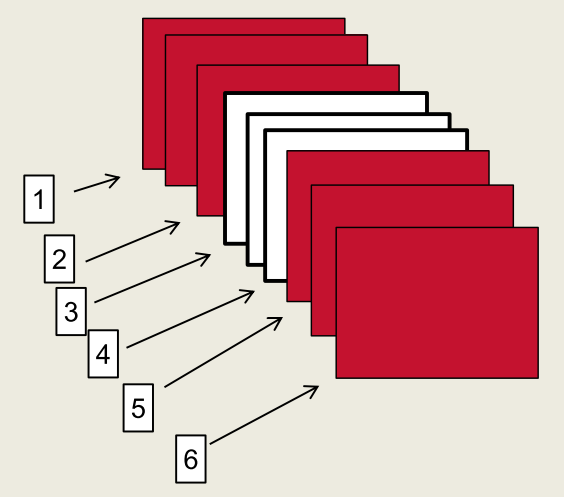
\includegraphics[width=0.4\textwidth]{./figures/eventos.png}
\caption{\small Ejemplo de una secuencia de eventos. Los cuadros coloreados y blancos indican eventos con poca o mucha relevancia, respectivamente. Los marcadores indican transiciones entre fases de poco y mucho interés. Obtenido de \cite{Kelley2014}.}
\label{img:sleep_eventos}
\end{figure}


%Ejemplo:
%At some location (cue), something big and orange (Tiger) moved from left to right resulting in pain (event)



%Abstraccion de episodios de manera declarativa simbolica... permite mejorar tiempos de busqueda


Además, este diseño permite que el sistema cambie su opinión sobre una evento, mediante aprendizaje reforzado. Si se repiten eventos, pero la consecuencia deja de ser la misma, entonces el sistema se acostumbra.

%\subsubsection{Frameworks relacionados}
%
%... ISAC \cite{Dodd2005}
%... MINERVA, LIDA, Neuronal,M SMRTI \cite{Jockel2008}
%... deficiencias de ISAC, EPIROME, \cite{Stachowicz2012}
%... sobre Tecuci, ISAC, SOAR y Ho \cite{Deutsch2008}
%... definir contenido de QWHAT \cite{Stachowicz2012}
%.. definicion de episodio \cite{Dodd2005}
%... diseno explicado de SONIA en RDF \cite{Vijayakumar2014}

%\todo[inline]{Sobre la memoria procedural}
%\subsection{Memoria Procedural}
%
%... procedural y CRAM \cite{Winkler2014}
%\cite{Winkler2014}

%...... habilidades y PM \cite{Salgado2012}


\subsection{Memoria Emocional}

La importancia de un evento se ve fuertemente influenciada por el estado emocional de una persona. Por lo tanto, la decisión de que almacenar o recordar depende de las emociones \cite{Deutsch2008}.

Su implementación requiere como mínimo de un mapeo entre estímulos percibidos por el robot y las sensaciones emocionales que estos generan. Dood et al. \cite{Dodd2005} propone el uso de la teoría emocional de reacciones de Haikonen, que considera a una emoción como una combinación de estímulos básicos. Las sensaciones elementales son: bienestar, malestar, dolor, placer e interés.

Dood et al. proponen implementar las sensaciones a partir de distintos estímulos medidos en un robot:

\begin{itemize}[topsep=0pt]
\setlength\itemsep{0.2em}
\item Actuador que se aproxima a sus límites de movimiento físico o de fuerza. 
\item Nivel de iluminación percibido.
\item Nivel de ruido acústico percibido.
\item Ausencia o presencia de humanos. Falta de interacción.
\item Cumplimiento de objetivos.
\item Cumplimiento de expectaciones.
\end{itemize}


Sistemas más avanzados, incluso pueden considerar la generación de reacciones emocionales, basándose en las sensaciones derivadas anteriormente. En la Figura \ref{img:emotional_haikonen} se muestran las reacciones generadas según el modelo de Haikonen. Además, estas se podrían reflejar en la personalidad del robot, por ejemplo, mediante gestos, vocabulario o nivel de aceptación para realizar una acción. Kasap et al. \cite{Kasap2010} utilizan un sistema llamado \textit{Emotion Engine}, para generar reacciones emocionales y simular cambios de personalidad de un robot, según las sensaciones percibidas.

\begin{figure}[H]
\centering
\begin{tabular}{| l | l |}
\hline
\rowcolor{gray!50}
Sensación Elemental & Reacción  \\ 
\hline Bueno: gusto, aroma & Aceptación, Acercar \\ 
\hline Malo: gusto, aroma & Rechazo, Alejar \\ 
\hline Dolor: autoinfligido  & Alejar, Desistir \\ 
\hline Dolor: agente externo & Agresión \\ 
\hline Dolor: sobre esfuerzo & Sumisión \\ 
\hline Placer & Mantener, Acercar \\ 
\hline Acierto & Mantener atención \\ 
\hline Desacierto & Migrar atención \\ 
\hline Novedad & Enfocar atención \\ 
\hline 
\end{tabular} 
\caption{\small Sensaciones elementales y sus reacciones correspondientes, según el modelo de Haikonen. Obtenido de \cite{Dodd2005}.}
\label{img:emotional_haikonen}
\end{figure}


Para su uso efectivo dentro de un esquema LTM, se espera que las sensaciones reportadas incluyan un nivel de intensidad. Según el nivel percibido en cada episodio, es posible clasificarlos entre eventos muy o poco relevantes. Los más relevantes tendrán mayor probabilidad de ser recuperados al recordar. Deutsch et al.  \cite{Deutsch2008} consideran que el la intensidad de las sensaciones es importante, pues permite evitar costos de búsqueda lineales dentro de todos los episodios almacenados. Por otro lado, Dood et al. proponen curvas de decaimiento para la importancia de los episodios, que permiten simular la pérdida de interés en los eventos.


%... + refs sobre emociones \cite{Deutsch2008}


%\todo[inline]{Resumen de dificultades ... diagrama o tabla.}


\subsection{Otros enfoques}

A continuación se presentan algunos estudios relacionados con aspectos de una memoria Ep-LTM que escapan de los requerimientos para este proyecto o que simplemente no son basados en la taxonomía de la memoria humana. Estos trabajos sólo se presentan a modo de completitud, pues no permiten resolver el objetivo de este proyecto, sino que sólo comprender otros enfoques y acercamientos a la solución. 

El sistema propuesto por Ho et al. \cite{Ho2009} busca modelar la memoria de forma suficientemente general, como para permitir el traspaso de los recuerdos de un robot a otro, independientemente de que el hardware sea distinto; El costo de esto, es que se reduce la personalización de cada robot. Ho et al. además aplican la teoría \textit{Roboética}, sugerida por Veruggio y Operto \cite{Veruggio2006}, de donde derivan restricciones de diseño, relativas al manejo de información privada de los usuarios.

En \cite{KimMinJoo2016}, Kim et al. plantean el uso de Deep Learning para modelar la memoria episódica y la planificación de acciones de manera holística. En su implementación, los procesos de codificación, almacenado y recuperación de episodios son manejados como uno solo. Los procesos de decaimiento y relevancia son abstraídos, para ser manejados automáticamente por la red.

Thorsten et al. \cite{Spexard2008} proponen una memoria LTM para el robot BIRON. En su trabajo, se abstraen de la clasificación entre memorias Ep-LTM y S-LTM, pues todos los datos de largo plazo almacenados por el robot son considerados LTM. La memoria almacena sólo datos de alto nivel, obtenidos tras el procesamiento de streams de datos básicos, como cámaras, micrófonos o actuadores. Los datos almacenados corresponden a un historial de percepciones y acciones de alto nivel realizadas, como: detecciones de objetos, interacciones verbales o la descripción de movimientos realizados. A pesar de su simplicidad, esta arquitectura centralizada permite reducir el las dependencias entre si de cada componente y reducir el ancho de banda utilizado para retransmitir la información entre procesos.


\todo[inline]{\cite{Pratama2014}}




\chapter{Aspectos Técnicos}\label{chapter:technical}

En este capítulo se describen los aspectos técnicos necesarios para comprender el diseño e implementación del proyecto. Primero, se presentan los componentes de software y hardware utilizados. Luego, se revisan algoritmos y conceptos computacionales utilizados en el trabajo.

%% =============================================================================

%% =============================================================================

%% =============================================================================

%% =============================================================================

%% =============================================================================

%% =============================================================================
%% =============================================================================
%% =============================================================================
\section{Componentes de software y hardware}
%% =============================================================================
%% =============================================================================
%% =============================================================================

A continuación se describen los componentes de software y hardware utilizados para el diseño e implementación del proyecto: Se hace una revisión breve de la base de datos MongoDB. Se revisan los conceptos utilizados sobre el framework robótico ROS. Se describe la librería SMACH, utilizada para la creación de máquinas de estado. Y finalmente, se presenta a Bender junto a los aspectos requeridos de su sistema operativo.

%% =============================================================================
%% =============================================================================
%% =============================================================================
\subsection{ROS}
%% =============================================================================
%% =============================================================================
%% =============================================================================

ROS \cite{ROS:2009}, acrónimo para Robot Operating System, es un proyecto que funciona como \textit{middleware} para aplicaciones robóticas, y permite resolver el problema de la comunicación entre procesos. Es una colección de herramientas, librerías y convenciones que buscan simplificar la tarea de crear comportamientos robóticos complejos y robustos, sin importar la plataforma robótica.

Fue originalmente creado por la organización WillowGarage en el 2008, y es mantenido actualmente por la Open Source Robotics Foundation (OSRF). Existe un ecosistema ROS, mantenido por la comunidad, y con cientos de módulos de software con soluciones a problemas específicos, los que pueden interconectarse para construir comportamientos más complejos. Por lo anterior, su uso se ha convertido en una práctica mundial, siendo adoptado incluso en soluciones industriales.

\subsubsection{Intraestructura}
%% =============================================================================

\paragraph{Nodo}
Es un programa ejecutable en ROS, enfocado en una tarea específica. Cada nodo puede establecer comunicación con otros a través de una interfaz ROS de tópicos o servicios.

\paragraph{Paquete}
Corresponde a un conjunto de nodos, junto a todos sus archivos necesarios para su compilación y ejecución. Cada paquete tiene asociado un nombre único en el sistema, junto a una lista de dependencias de otros paquetes. ROS provee conjunto estándar de paquetes y librerías enfocados en diversos aspectos de la robótica, que en conjunto a los paquetes mantenidos por la comunidad, permiten simplificar la construcción y mantenimiento de un robot.

\paragraph{Distribuciones} 
Una distribución es un conjunto versionado de paquetes ROS. Su propósito es permitir que los desarrolladores trabajen en un conjunto relativamente estable de dependencias, hasta que puedan avanzar a la siguiente versión. Se libera una distribución anualmente, enfocada a una versión  LTS\footnote{LTS es un acrónimo para Long-Term-Support. Una versión LTS de un software indica que éste contará con soporte a largo plazo, es decir, durante un periodo mayor a su periodo normal de vigencia.} de Ubuntu, y las versiones pares de ROS también se consideran LTS y mantienen soporte por 5 años.

\paragraph{Lenguajes de programación} ROS provee librerías oficiales para escribir nodos en los lenguajes C++ (\texttt{roscpp}\footnote{Documentación oficial de \texttt{roscpp}: \url{http://wiki.ros.org/roscpp}.}), Python (\texttt{rospy}\footnote{Documentación oficial de \texttt{rospy}: \url{http://wiki.ros.org/rospy}.}) y Common Lisp (\texttt{roslisp}\footnote{Documentación oficial de \texttt{roslisp}: \url{http://wiki.ros.org/roslisp}.}), junto a librerías experimentales para otros lenguajes.

\subsubsection{Comunicación}
%% =============================================================================

\paragraph{ROS master} Es el servidor central de ROS y provee servicios de registro al resto de los nodos. Mantiene una lista de los tópicos, servicios y parámetros disponibles, que han registrado los nodos activos. Su principal funcionalidad es permitir que cada nodo pueda encontrar a los otros. Una vez establecida la comunicación, los nodos se comunican en una red P2P\footnote{En una red P2P (peer-to-peer) los participantes se comunican total o parcialmente sin requerir un servidor intermediario.}. Comúnmente la comunicación en ROS se realiza mediante el protocolo HTTP, bajo un transporte TCP, sin embargo, los nodos pueden ser configurados para utilizar un transporte basado en UDP. Por lo tanto, ROS permite el manejo de nodos de manera distribuida, siempre que cada máquina tenga acceso a la red del computador ejecutando el ROS master.

\paragraph{Mensaje} Es una estructura de datos utilizada para comunicar un nodo con otro. Se definen en un mensaje de tipo \texttt{.msg}, a partir de tipos de dato básicos en ROS y otros mensajes. Durante la compilación se genera el código para poder utilizarlos mediante las librerías ROS de cada lenguaje de programación disponible.

\paragraph{Tópico} Permite que los nodos de comuniquen a través de mensajes, y está basado en el patrón de diseño observador. Cada tópico es un canal de comunicación que transmite mensajes ROS de un tipo predefinido. Cada nodo puede publicar simultáneamente en uno o más tópicos. Cada nodo puede suscribirse a los tópicos que desee, siendo notificado por cada mensaje entrante. Esto se describe en el diagrama de la Figura \ref{img:ros-topic}.

\begin{figure}[!h]
	\centering
	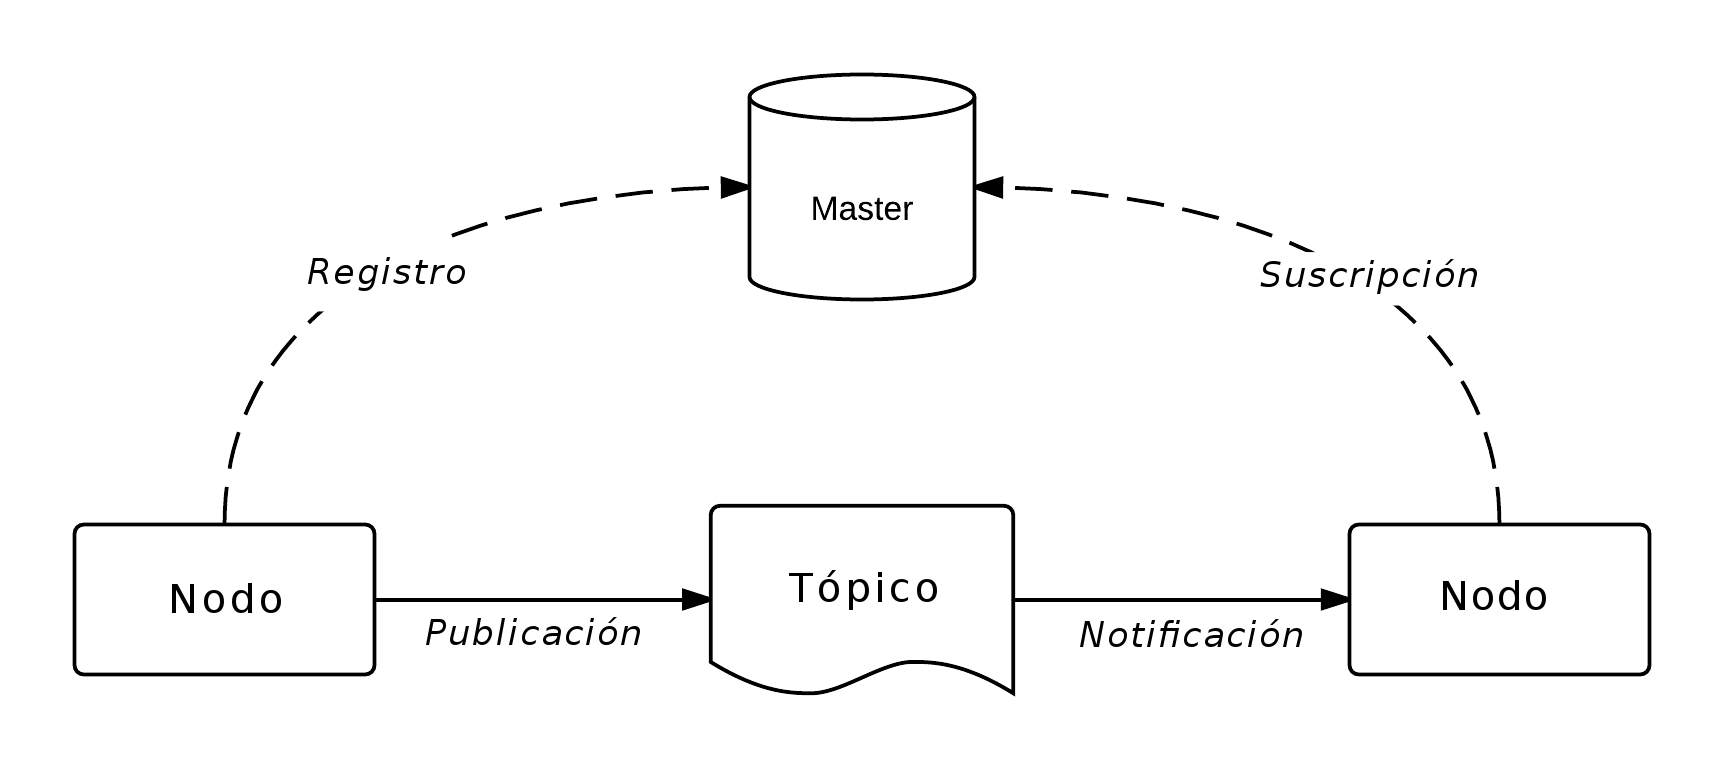
\includegraphics[width=0.8\textwidth]{ROS-master-node-topic-esp.png}
	\caption{\small Diagrama de la comunicación mediante tópicos en ROS. El ROS master se encarga de establecer el proceso de comunicación entre los nodos involucrados. Luego los nodos se comunican {\bfseries unidireccionalmente} usando el tópico establecido.}
	\label{img:ros-topic}
\end{figure}

\paragraph{Servicios} Es una forma de comunicación cliente-servidor de carácter síncrono. Se construyen a partir de una estructura de datos de tipo \texttt{.srv}, que especifica mensajes ROS de petición y respuesta, disponible tras la compilación. Cada nodo (servidor) puede proveer uno o más servicios. Cada nodo (cliente) puede enviar peticiones al servidor. Las peticiones son de carácter bloqueante, hasta que una respuesta desde el servidor sea recibida.

\paragraph{Acciones} Esta forma de comunicación se construye a partir de tópicos y servicios, mediante la librería \texttt{actionlib} \footnote{Documentación oficial de \texttt{actionlib}: \url{http://wiki.ros.org/actionlib}.}. Está enfocada en la resolución de tareas de largo plazo, y funciona a través de metas solicitadas por el cliente. El servidor mantiene una máquina de estados que recibe peticiones (servicio) e informa constantemente sobre el estado del proceso y su resultado (tópicos). La estructura de datos utilizada es de tipo \texttt{.action}, que especifica mensajes ROS para la petición, el \textit{feedback} y el resultado.

\paragraph{Servidor de parámetros} ROS provee un servidor para almacenar, modificar y obtener parámetros compartidos entre los nodos. Éstos permiten la configuración del programa sin tener que recompilar el código, y funcionan como el estándar para el manejo de parámetros. La configuración por defecto puede ser especificada en archivos usando el formato YAML.


\subsubsection{Herramientas}
%% =============================================================================

\paragraph{Pluginlib} Es un paquete oficial de ROS\footnote{Documentación oficial de \texttt{pluginlib}: \url{http://wiki.ros.org/pluginlib}.} que provee herramientas para escribir y cargar plugins dinámicamente en nodos C++. La librería permite delegar la implementación de funcionalidades específicas a los usuarios. El nodo que ocupará el plugin debe definir una clase abstracta a ser implementada. Mientras que los paquetes proveedores deben registrar las librerías con sus implementaciones, para que los plugins queden disponibles en el sistema.

\paragraph{Roslaunch} La librería \texttt{roslaunch}\footnote{Documentación oficial de \texttt{roslaunch}: \url{http://wiki.ros.org/roslaunch}.} es una herramienta que permite la ejecución y configuración de múltiples nodos, a través de sólo un comando en la consola del sistema. Utiliza archivos en formato XML y con extensión \texttt{.launch}, donde se define un árbol de nodos y otros archivos \textit{launch} a ser ejecutados. Esta herramienta permite modularizar la ejecución de un sistema robótico complejo, compuesto generalmente por decenas de nodos.

%\paragraph{Rviz}
%\paragraph{Rosbag} (probablemente se ocupará para test suite)


%% =============================================================================
%% =============================================================================
%% =============================================================================
\subsection{MongoDB}\label{sec:mongodb}
%% =============================================================================
%% =============================================================================
%% =============================================================================

\subsubsection{Conceptos:}

MongoDB es una base de datos no relacional orientada a documentos tipo JSON, donde los campos pueden variar de documento a documento y la estructura de datos puede ser modificada en el tiempo \cite{MongoDB}. MongoDB está diseñada para funcionar de manera distribuida, proveer alta disponibilidad, escalamiento horizontal y distribución geográfica. Es una base de datos gratis y de código libre, publicada bajo la licencia GNU AGPL.

MongoDB representa documentos JSON en un formato binario denominado BSON. BSON extiende JSON a través de nuevos tipos de datos, introduce campos ordenados y está diseñado para proveer eficiencia al codificar y decodificar la información en distintos lenguajes. 

Los documentos son organizados en \textit{colecciones}, cada una destinada a almacenar información asociada a un concepto particular. MongoDB provee funcionalidades para consultas, indexado y realizar agregaciones de los datos almacenados.

MongoDB provee drivers para diversos lenguajes de programación, entre ellos C++, Java y Python. Para este proyecto, el driver de interés es el de C++11\footnote{Documentación del driver de MongoDB para C++:  \url{http://mongodb.github.io/mongo-cxx-driver/}.}.

En su configuración por defecto, el servidor de MongoDB soporta documentos de hasta 16MB de tamaño, lo que restringe la información a almacenar, pero permite mantener acotados los costos de las operaciones sobre la base de datos. Este límite puede ser removido al modificar el algoritmo de almacenamiento a GridFS, que divide documentos grandes en subdocumentos menores a 16MB, para ser tratados normalmente.

\subsubsection{Interfaz ROS:}

MongoDB es una de las dependencias de \textit{MoveIt!}\footnote{Documentación oficial de MoveIt!: \url{https://moveit.ros.org/}.}, librería estándar utilizada para la manipulación de objetos, de uso extendido en la comunidad robótica. Por lo tanto, MongoDB ya está instalada y funcionando en muchos robots de servicio basados en ROS. 

El equipo desarrollador de MoveIt! y sus paquetes ROS relacionados mantiene el paquete \texttt{warehouse\_ros\_mongo}\footnote{El paquete ROS \texttt{warehouse\_ros\_mongo} está disponible en: \url{https://github.com/ros-planning/warehouse\_ros\_mongo}.}, que provee una interfaz ROS al driver en C++ para MongoDB. MoveIt! y sus dependencias son consideradas estables, al menos durante el periodo de la última distribución ROS, con fecha de caducidad para el 2023.

\texttt{warehouse\_ros\_mongo} permite definir colecciones destinadas a almacenar mensajes ROS, de manera binaria. Cada documento es construido a partir del mensaje ROS serializado (mediante su API ROS), sumado a un conjunto de metadatos utilizados para la definición de índices y consultas. Actualmente, la API sólo soporta la definición de metadatos de los tipos \texttt{bool}, \texttt{int}, \texttt{double} y \texttt{std::string} en C++.


%% =============================================================================
%% =============================================================================
%% =============================================================================
\subsection{SMACH}
%% =============================================================================
%% =============================================================================
%% =============================================================================

SMACH es una librería en Python para la creación y ejecución de máquinas de estado. Permite crear rápidamente comportamientos robóticos complejos, basados en capacidades de alto nivel de un robot. Está diseñada para ser independiente de ROS, pero provee una interfaz para su uso. Se puede encontrar en el conjunto de paquetes ROS denominado \texttt{executive\_smach}\footnote{Documentación oficial de SMACH disponible en: \url{http://wiki.ros.org/smach}.}.

\begin{figure}[!h]
	\centering
	\includegraphics[width=0.8\textwidth]{smach-sample.png}
	\caption{\small Ejemplo de máquina de estado construida en SMACH para la representación de una rutina de carga automática de baterías. Obtenido desde la documentación oficial.}
	\label{img:SMACH-sample}
	\todounsure{Es necesario poner la figura en español??}
\end{figure}



En SMACH una maquina de estado está compuesta por un conjunto de estados y sus transiciones. La librería soporta anidamiento, por lo que cualquier estado puede ser reemplazado por otra máquina de estado disponible. Cada estado debe proveer una función \texttt{execute} a ser ejecutada cuando esté activo. En la Figura \ref{img:SMACH-sample} se presenta un ejemplo de un comportamiento robótico complejo implementado en SMACH, que representa el proceso de recarga de baterías en un robot. Según las condiciones encontradas se activarán distintas transiciones, pero en el caso básico la rutina es la siguiente: El robot navega a la estación de carga, se posiciona, manipula el conector, se conecta y espera.

%% =============================================================================
%% =============================================================================
%% =============================================================================
\subsection{UChile ROS Framework}\label{sec:URF}
%% =============================================================================
%% =============================================================================
%% =============================================================================

\subsubsection{Conceptos}

UChile ROS Framework (URF) hace referencia al sistema de software desarrollado en el laboratorio de robótica del Departamento de Ingeniería Eléctrica de la Universidad de Chile, para sus robots de servicio. El sistema cuenta con 10 años de desarrollo y está orientado a cumplir los requisitos de la competencia RoboCup en su categoría @Home.

URF está construido sobre ROS y en una estructura de 4 capas:
\begin{enumerate}
\item La primera capa contiene todas las dependencias del sistema, ya sean de ROS o no. Es la única capa que contiene sólo código externo.
\item  Sobre la primera capa se monta una capa ROS de bajo nivel, con herramientas y librerías comunes, sumado a los drivers necesarios para manejar cada robot (módulos de \textit{Hardware} en la Figura \ref{img:URF}).
\item La capa intermedia alberga capacidades robóticas avanzadas, relacionadas a percepción robótica, manipulación de objetos, navegación autónoma e interacción Humano-Robot (sección \textit{Módulos ROS} del diagrama).
\item La última capa \textit{de alto nivel} es desarrollada en Python, con interfaces para el uso de las capacidades de menor nivel, y es utilizada para la elaboración de maquinas de estado y comportamientos robóticos complejos mediante SMACH (cuadros \textit{Interfaz ROS-python} y \textit{State Machine} del diagrama).
\end{enumerate}

\begin{figure}[!h]
	\centering
	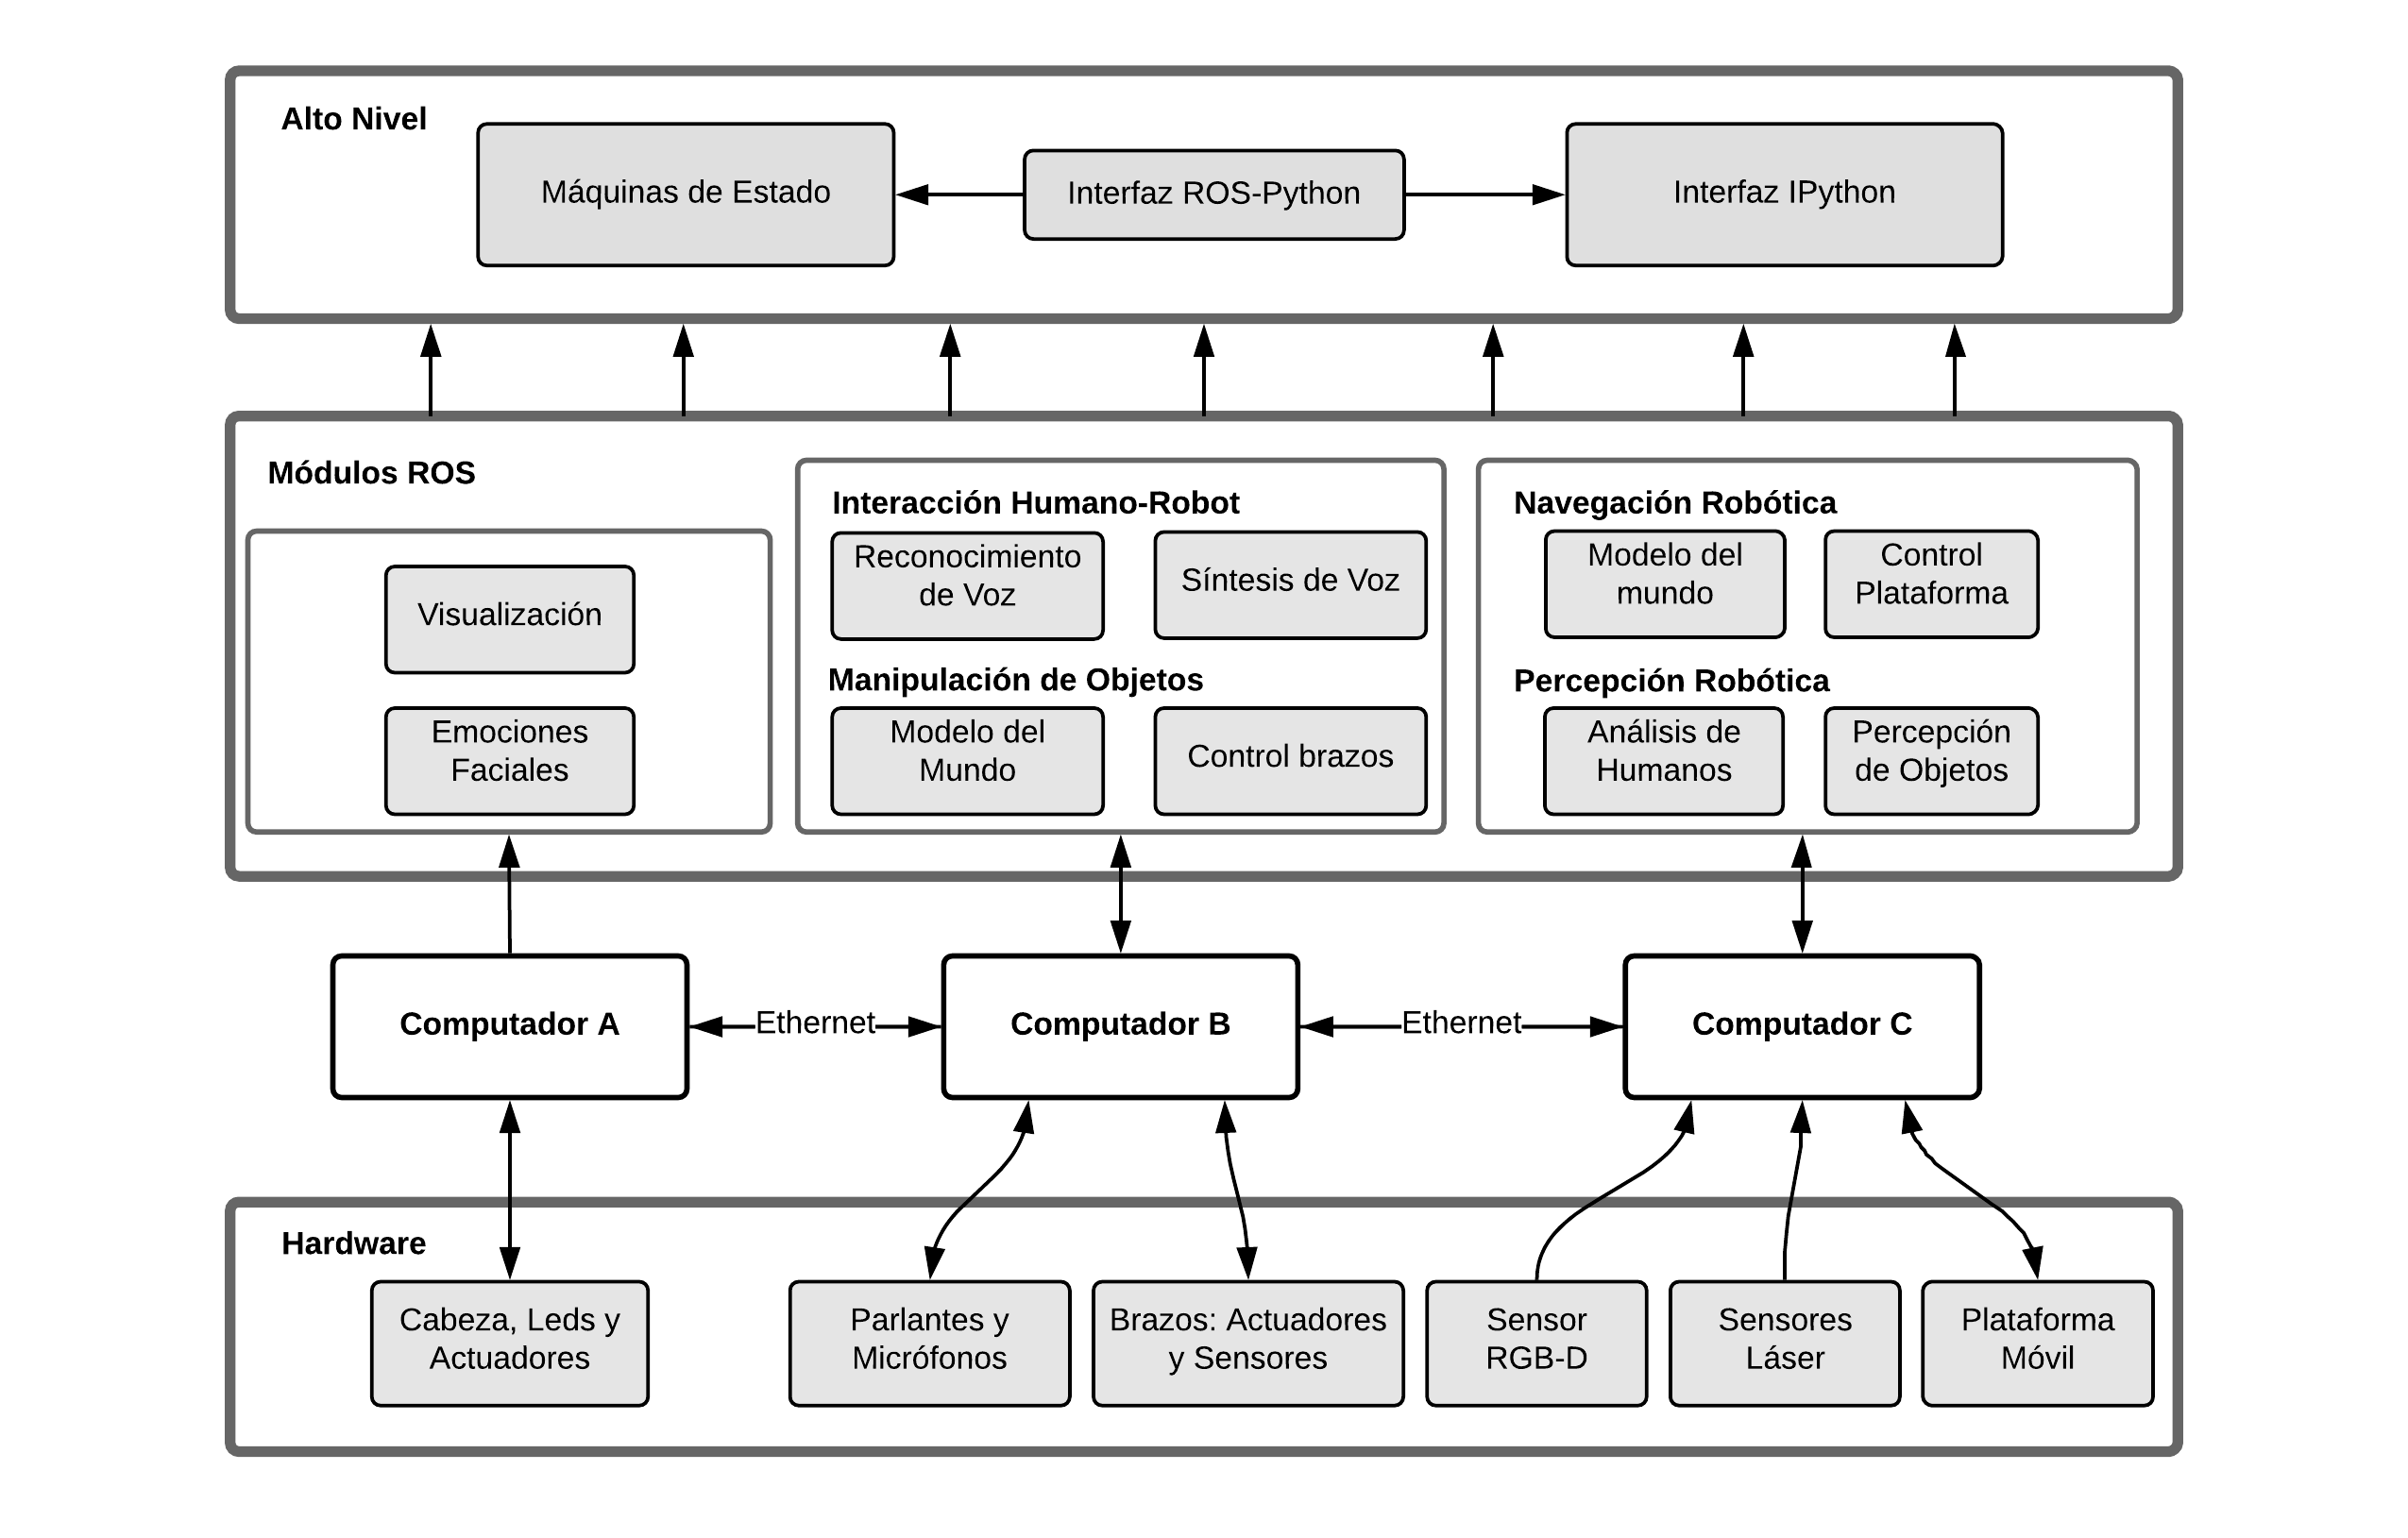
\includegraphics[width=0.8\textwidth]{URF-esp.png}
	\caption{\small Diagrama de UChile ROS Framework utilizado en el robot Bender.}
	\label{img:URF}
\end{figure}

Todos los módulos de URF son de código libre, a excepción de los algoritmos relacionados con percepción y la interfaz de alto nivel. El código se almacena públicamente en la organización \textit{uchile-robotics} en GitHub\footnote{Organización \textit{uchile-robotics} y URF en GitHub: \url{https://github.com/uchile-robotics}}.


\subsubsection{Memoria a corto y largo plazo}
%% =============================================================================

En un robot implementado sobre URF es posible acceder a la información compartida por sus procesos. Cualquier módulo ROS en el sistema tiene acceso a los datos extraídos desde sensores y luego generados en post-procesamientos, junto al acceso para controlar el hardware.

Existen algunas formas de memoria implementadas en URF, comparables a los conceptos definidos para la memoria humana. También se pueden dividir en de corto y largo plazo:

Como STM, se puede definir como memoria de trabajo a todo el flujo de información presente durante la ejecución del robot. Lo que incluye datos sensados, procesamientos y acciones realizadas. Generalmente tales datos no son almacenados para posteriores ejecuciones.

A manera de LTM, se puede encontrar una memoria procedural, relacionada con todo el conocimiento almacenado que posee el robot para cumplir ciertas tareas. Caen en esta categoría: modelos para percepción robótica, modelos para reconocimiento de voz y patrones, bases de datos de movimientos precalculados para manipular objetos y acciones predefinidas que se utilizan para controlar el robot.

También se pueden encontrar especializaciones de memoria LTM semántica. Ejemplos de esto son: El mapa que se conoce del entorno, junto a los lugares y objetos anotados en él. Diccionarios con información anotada sobre entidades y sus características, cómo personas y objetos. Bases de datos con imágenes anotadas para el reconocimiento de objetos y personas. 

Sin embargo, en URF no existen formas de memoria emocional ni episódica de largo plazo. Luego, toda interacción realizada por los robots está limitada a la información obtenida desde el inicio al término de cada rutina.


%% =============================================================================
%% =============================================================================
%% =============================================================================
\subsection{Bender}
%% =============================================================================
%% =============================================================================
%% =============================================================================
%% -----------------------------------------------------------------------------

Bender es un robot humanoide creado el año 2007 en el laboratorio de robótica del Departamento de Ingeniería Eléctrica de la Universidad de Chile. El equipo UChile Homebreakers es el encargado de su desarrollo y  su objetivo es ser un mayordomo para el hogar, funcionando de manera autónoma para apoyar en tales labores \cite{uchile-robotics}.

En cuanto a actuadores, el robot cuenta con 2 brazos antropomórficos de 6 grados de libertad cada uno, una base móvil diferencial Pioneer 3-AT, un cuello que permite rotaciones en dos ejes cartesianos; pudiendo imitar gestos de asentimiento y negación, y finalmente, una cabeza que puede mostrar expresiones faciales mediante movimientos de su boca, orejas, cejas y cambios de colores alrededor de los ojos.

El robot cuenta con los siguientes sensores: un laser Hokuyo UTM-30LX, un laser Hokuyo URG-04LX-UG01, un micrófono M-Audio Producer USB y una cámara de profundidad ASUS Xtion Pro.

El software de Bender está basado en el framework URF. Su arquitectura de software utiliza  ROS para el manejo de componentes de bajo y medio nivel. La capa de alto nivel, escrita en python, se abstrae de ROS y permite la creación de comportamientos complejos mediante máquinas de estado. Todos los módulos que interactúan con sensores y actuadores están implementados en ROS.

\begin{figure}[!h]
	\centering
	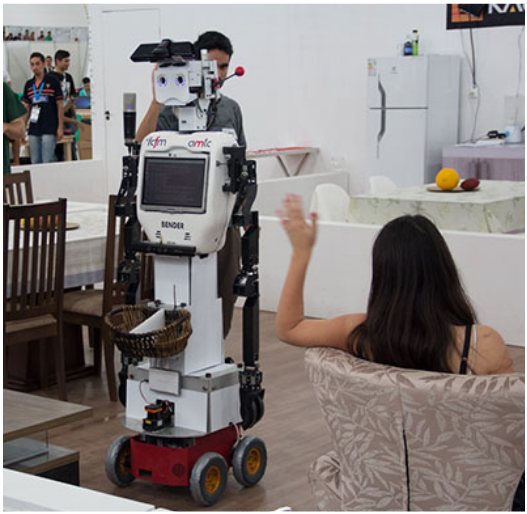
\includegraphics[width=0.4\textwidth]{bender.png}
	\caption{\small Robot Bender en competencia RoboCup@Home 2015.}
	\label{img:bender}
\end{figure}

\todoimprove{Sobre la cantidad de paquetes ROS, nodos, tópicos y mensajes disponibles.}
\todoimprove{API a ocupar para acceder a datos del robot.}


%% =============================================================================

%% =============================================================================

%% =============================================================================

%% =============================================================================

%% =============================================================================

%% =============================================================================

%% =============================================================================
%% =============================================================================
%% =============================================================================
\section{Algoritmos y conceptos computacionales}
%% =============================================================================
%% =============================================================================
%% =============================================================================
\todounsure{TODA ESTA SECCIÓN PODRÍA SER ELIMINADA....????}
\todounsure{convex hull}
\todounsure{procesamiento de imágenes: degradación de streams}
\todounsure{Algs utilizados para emociones implementadas en robot}
\todounsure{Sistemas de coordenadas?? Frames?}





\chapter{Metodología}\label{chapter:metodologia}

En este capítulo se presenta la metodología a utilizar para el desarrollo del trabajo de título. En primer lugar se presentan las alternativas de solución evaluadas para el proyecto, haciendo énfasis en la factibilidad de la propuesta. Para luego, describir la planificación de tareas a realizar durante el segundo periodo del proceso, sustentadas en las soluciones propuestas. Finalmente, se presenta una carta gantt con los periodos de trabajo estimados.


%\section{Requerimientos para un robot doméstico}
%
%\todo[inline]{Sobre los requerimientos en específico para robots domésticos}
%
%Para entender el alcance del trabajo, en cuanto a qué es lo que se espera del sistema, a continuación se listan algunas capacidades de los robots domésticos. Un robot de compañía y asistencia tiene, pero no se limita a las siguientes tareas:
%\begin{itemize}[topsep=0pt]
%\setlength\itemsep{0.2em}
%\item Interacción amistosa con humanos.
%\item Ayudar a recordar y organizar tareas.
%\item Cooperar con la realización de un procedimiento.
%\item Guiar y seguir a personas.
%\item Recordar información y entidades.
%\end{itemize}
%\bigskip
%
%Algunas tareas que robots domésticos de tipo mayordomo deben ejecutar son:
%\begin{itemize}[topsep=0pt]
%\setlength\itemsep{0.2em}
%\item Ofrecer comida y bebestibles.
%\item Preparación de comida.
%\item Ordenar y limpiar el hogar.
%\end{itemize}
%\bigskip

%\subsubsection{Requerimientos para robots domésticos}
%
%En términos de LTM, un robot doméstico necesita poder recordar los siguientes conocimientos:
%
%... \todo[inline]{tareas de un robot de servicio}
%\begin{itemize}
%\item 
%\end{itemize}
%
%... casos de uso e inferencia \cite{Vijayakumar2014}
%
%... artificial companion PAG 13 \cite{Vijayakumar2014}
%


\section{Propuesta de Solución}

%Temas a resolver:
%
%- modelo de memoria a utilizar
%- arquitectura
%- consolidación
%- base de datos
%- demostracion 
%- emociones
%- inferencia

La primera parte consiste en definir un conjunto de consultas que un robot doméstico debe responder a partir de la memoria. Esto estará baso en los requerimientos mostrados en la Sección \ref{sec:domestic_robots}. Particularmente, el foco del trabajo, será generar una memoria LTM adecuada a las interacciones que realizaría el robot Bender. A partir de las consultas se definirán los modelos semánticos a considerar y sus características. 

El diseño de la memoria LTM estará basado en los 11 requerimientos de diseño mostrados en la sección \ref{sec:ltm_exp}. Además se basará en la taxonomía de la memoria humana, de manera similar a los trabajos desarrollados por Vijayakumar  \cite{Vijayakumar2014} y Sánchez et al. \cite{Sanchez:2015}.

El algoritmo a utilizar para la consolidación de STM en LTM no está claro aún y debe ser estudiado. Esta es la parte más relevante del trabajo, donde se tomarán las decisiones de diseño definitivas. No existe un consenso al respecto en la literatura, pero un primer acercamiento será basado en la propuesta de Sánchez et al.  \cite{Sanchez:2015}, para la definición de episodios, sumado al trabajo de Kelley  \cite{Kelley2014} para la selección de qué eventos almacenar y cómo procesarlos.

Una vez definido el proceso de consolidación, queda definir una arquitectura de software. Se propone basar el desarrollo en el software KnowRob, pues fue diseñado para manejar memoria semántica y procedural, además de proveer funcionalidades para realizar inferencias. Por su estructura, se cree que la Ep-LTM puede ser almacenada como si fuese memoria semántica. Entonces, el desafío se centra en poder agregar el soporte para memoria episódica al sistema. KnowRob ha sido descargado y se ha comprobado el funcionamiento de sus módulos principales.

En cuanto a la integración de KnowRob y la Ep-LTM en URF, se cree que se deberá agregar un nuevo módulo al sistema. De acuerdo a la Figura \ref{img:URF}, se debería agregar la Ep-LTM como un componente en la \textit{capa de alto nivel}, pues es donde se manejan las máquinas de estado del robot y el único lugar donde se podrían abstraer los conceptos de evento y episodio. Las capas de menor nivel sólo se encargan de proveer funcionalidades para construir los comportamientos ejecutados por el robot. Se debe diseñar la solución final, pero a priori, la Ep-LTM debe tener acceso a todos los componentes de la \textit{capa de alto nivel}. Además, se debe considerar que una futura implementación de memoria emocional debería interactuar directamente con el hardware del robot. 


Finalmente, se debe implementar un servicio que escuche constantemente los eventos ocurridos en el sistema, los analice y almacene recuerdos. Luego se debe implementar una demostración del uso de los datos recopilados.

No se trabajará en la inferencia de información, sino que sólo se aprovechará de que KnowRob provee herramientas para ello, lo que asegura que en un futuro se podrán agregar inferencias al sistema. La memoria emocional sólo será considerada para la etapa de diseño, pero su implementación no es requerida.


La demostración será definida como un conjunto de validaciones que permitan corroborar el funcionamiento del sistema. Por lo tanto, esta será implementada incrementalmente, para validar cada desarrollo del trabajo. Las validaciones más relevantes tienen que ver con la capacidad del sistema para responder las consultas episódicas seleccionadas para robots domésticos.

%\subitem - Consultas episódicas: ``Qué hiciste ayer y cómo?'', ``Qué pasó hace 1 mes?''.
%\subitem - Consultas semánticas: ``Qué ha cambiado en la habitación?'', ``Describe un humano que conozcas.''.


% Una vez definido el proceso de consolidación, se puede implementar el servicio que recopile información constantemente. éste podría acceder a la información que genera el robot durante sus rutinas, una forma de STM básica, mediante sus interfaces ROS.

% Respaldos
%Capacidad de generar respaldos de la memoria y recuperación de éstos. Mezcla del respaldo con memoria ya existente.


%\subsubsection{OTROS}
%\begin{itemize}
%\item Visualizador de la memoria e interfaz para facilitar gestión de los recuerdos por parte de un operador.
%\item Migración de memoria a otros robots.
%\item Memoria compartida entre robots.
%\item Uso de memoria emocional para dar personalidad y reflejar estado de ánimo.
%\item Complementar recopilación de información e inferencia mediante información WEB.
%\item Uso de servicio web para análisis de frases e intenciones, para responder preguntas en lenguaje natural.
%\end{itemize}


\section{Planificación}

Durante el trabajo de título se propone seguir una estrategia incremental de desarrollo de software, que considere cada uno de los objetivos específicos. La demostración es de carácter transversal al proyecto, pues se utilizará como medio de validación de cada parte del trabajo. Considerando la solución propuesta, se tienen las siguientes etapas del proyecto:
\begin{enumerate}[topsep=10pt]
\setlength\itemsep{0.2em}
\item Definir consultas a responder por un robot doméstico. Seleccionar entidades a ser modeladas, acordes a las consultas.

\item Diseñar el algoritmo de consolidación de STM en LTM.

\item Implementación de componente Ep-LTM para KnowRob.

\item Integración de KnowRob en Bender

\item Servicio para recopilación continua de recuerdos.

\end{enumerate}

Los tiempos estimados de trabajo para cada una de las tareas anteriores se presentan en la siguiente carta Gantt. La resolución de los tiempos es a periodos de 15 días.

\begin{center}
\scalebox{1.2}[1.0]{
%\rotatebox{0}{
\boxed{
\begin{gantt}{8}{9}
	\begin{ganttitle}
		\titleelement{Ago.}{1}
		\titleelement{Sept.}{2}
		\titleelement{Oct.}{2}
		\titleelement{Nov.}{2}
		\titleelement{Dic.}{2}
    \end{ganttitle}
    \ganttbar[color=cyan]{\small Consultas y Modelos}{0}{2}
    \ganttbar[color=cyan]{\small Algoritmo de Consolidación}{1}{3}
    \ganttbar[color=red]{\small Ep-LTM en KnowRob}{3}{2}
    \ganttbar[color=magenta]{\small Integración en URF}{5}{2}
    \ganttbar[color=yellow]{\small Generación de Recuerdos}{6}{3}
	\ganttbar[color=orange]{\small Demo y Validación}{3}{6}
	\ganttbar[color=gray]{\small Escritura}{1}{8}
\end{gantt}
%}
}}
\end{center}




\bibliographystyle{IEEEtran}
\bibliography{IEEEabrv,bibliography}


\end{document}